
 % برای جدول‌های با عرض قابل تنظیم
   % برای استفاده از فونت‌های فارسی
% برای پشتیبانی از زبان‌های راست به چپ
% \usepackage{array}       % برای ستون‌های m{}
% \usepackage{enumitem}    % برای تنظیم فاصله لیست‌ها
% \usepackage{booktabs}    % برای خطوط زیباتر در جدول‌ها


% تعریف یک ستون m{عرض} با مرکزچین کردن افقی
\newcolumntype{M}[1]{>{\centering\arraybackslash}m{#1}}





\chapter{نتایج}

%------------------------------------------------------------------------------------------------
\section{معرفی مجموعه داده}
\subsection{ضرورت انتخاب دیتاست مناسب}
انتخاب دیتاست مناسب یکی از حیاتی‌ترین مراحل است. این انتخاب مستقیماً بر دقت و موفقیت مدل‌های یادگیری ماشین تأثیر می‌گذارد. یک دیتاست ایده‌آل باید از تنوع بالایی در شرایط محیطی برخوردار باشد؛ به عنوان مثال، شرایطی مانند نورپردازی، زاویه دید و وضوح تصاویر باید به گونه‌ای متنوع باشند که مدل بتواند عملکردی قابل قبول در محیط‌های واقعی داشته باشد.

جامعیت و تعداد نمونه‌های کافی برای هر کلاس از علائم راهنمایی و رانندگی نیز از اهمیت بالایی برخوردار است. این ویژگی به مدل امکان می‌دهد تا انواع مختلف علائم را به درستی یاد بگیرد و دقت خود را در پیش‌بینی بهبود بخشد. علاوه بر این، ساختار استاندارد دیتاست و انوتیشن‌های دقیق نظیر جعبه‌های محصور\LTRfootnote{Bounding Boxes} یا ماسک‌های تفکیکی\LTRfootnote{Segmentation Masks} می‌توانند فرآیند آموزش و ارزیابی را تسهیل کنند. پذیرش گسترده دیتاست در جامعه علمی نیز به عنوان یک شاخص کیفیت و اعتبار، انتخاب آن را برای تحقیقات تسهیل می‌کند. 

تعادل کلاس‌ها و پوشش جغرافیایی گسترده دیتاست نقش مهمی در جلوگیری از تعصب مدل به کلاس‌های پرتعداد ایفا می‌کنند. در نهایت، دسترسی آزاد و مجوزهای مناسب استفاده از دیتاست، امکان بهره‌برداری در پروژه‌های آتی را فراهم می‌کند. 

\section{بررسی و تحلیل دیتاست‌ها}

در ادامه، به بررسی و تحلیل چندین دیتاست معتبر در حوزه شناسایی علائم راهنمایی و رانندگی می‌پردازیم. هر یک از این دیتاست‌ها دارای ویژگی‌ها و کاربردهای خاص خود هستند که آن‌ها را برای پروژه‌های مختلف مناسب می‌سازد. 

دیتاست \textbf{GTSRB\LTRfootnote{German Traffic Sign Recognition Benchmark}} یکی از پرکاربردترین مجموعه داده‌ها در این زمینه است که شامل \lr{50,000} تصویر از \lr{43} کلاس مختلف علائم می‌باشد. تنوع بالای این دیتاست در شرایط نوری و زاویه دید به مدل‌ها امکان می‌دهد تا با تغییرات محیطی مختلف سازگار شوند و دقت بالایی در شناسایی علائم داشته باشند. کیفیت بالای انوتیشن‌های این دیتاست، که شامل جعبه‌های محصور است، فرآیند آموزش مدل‌ها را تسهیل کرده و دقت شناسایی را افزایش می‌دهد.

دیتاست \textbf{\lr{TT100K}\LTRfootnote{Traffic Sign Dataset 100K}} با بیش از \lr{100,000} تصویر و \lr{100} کلاس مختلف، یکی از بزرگترین دیتاست‌ها در این حوزه محسوب می‌شود. این دیتاست به دلیل تنوع بالای شرایط محیطی و تعداد زیاد نمونه‌ها برای پروژه‌هایی که نیاز به داده‌های گسترده دارند بسیار مناسب است. با این حال، تمرکز جغرافیایی این دیتاست بر روی کشور چین می‌تواند در تعمیم مدل به سایر مناطق چالش‌هایی ایجاد کند و ممکن است باعث کاهش دقت مدل‌ها در شناسایی علائم راهنمایی و رانندگی در مناطق دیگر شود.

دیتاست \textbf{LISA\LTRfootnote{Laboratory for Intelligent and Safe Automobiles}} شامل حدود \lr{25,000} تصویر از \lr{47} کلاس مختلف علائم است. این دیتاست به دلیل تعادل نسبی بین کلاس‌ها و کیفیت مناسب تصاویر، برای پروژه‌هایی که بر روی علائم در محیط‌های کنترل‌شده تمرکز دارند، بسیار مناسب است. انوتیشن‌های دقیق این دیتاست، فرآیند آموزش مدل‌ها را بهبود بخشیده و دقت شناسایی را افزایش می‌دهد.

دیتاست \textbf{Mapillary} با داشتن بیش از \lr{100,000} تصویر و \lr{600} کلاس مختلف، تنوع جغرافیایی و محیطی بسیار بالایی ارائه می‌دهد. این دیتاست برای پروژه‌های بین‌المللی و مطالعاتی که نیاز به داده‌های گسترده و متنوع دارند، گزینه‌ای ایده‌آل است. انوتیشن‌های دقیق و جامع این دیتاست، امکان آموزش مدل‌های پیچیده‌تر و دقیق‌تر را فراهم می‌آورد.

دیتاست \textbf{BelgiumTS\LTRfootnote{Belgium Traffic Sign Dataset}} شامل حدود \lr{7,000} تصویر از \lr{108} کلاس مختلف علائم است. اگرچه کیفیت تصویری بالایی دارد، اما به دلیل محدودیت در تعداد نمونه‌ها و تنوع محیطی کمتر، برای پروژه‌هایی که نیاز به تنوع و داده‌های گسترده دارند، مناسب نیست. این دیتاست بیشتر برای پروژه‌های کوچک‌تر و تحقیقات مقدماتی کاربرد دارد.


علاوه بر دیتاست‌های فوق، تکنولوژی‌های نوینی مانند \textbf{ترنسفورمر های بینایی  \LTRfootnote{Vision Transformers}} و روش‌های ترکیبی بین شبکه‌های عصبی کانولوشنی و ترنسفورمرها نیازمند دیتاست‌هایی با ساختار مناسب و ویژگی‌های دقیق هستند. دیتاست‌هایی که توانسته‌اند نیازهای این مدل‌های پیشرفته را برآورده کنند، نقش مهمی در پیشرفت تحقیقات و بهبود عملکرد سیستم‌های شناسایی علائم راهنمایی و رانندگی ایفا می‌کنند. به عنوان مثال، دیتاست‌های با انوتیشن‌های دقیق و تنوع بالا، امکان استفاده بهینه از مدل‌های ترنسفورمر را فراهم می‌آورند و باعث افزایش دقت و سرعت شناسایی می‌شوند.









\begin{latin}

\begin{table}[h!]
\centering
\resizebox{\textwidth}{!}{%
\begin{tabular}{|l|c|c|c|c|c|c|c|}
\hline
\textbf{Dataset} & \textbf{\#Images} & \textbf{\#Classes} & \textbf{\#Signs} & \textbf{Attributes} & \textbf{Region} & \textbf{BBoxes} & \textbf{Unique} \\
\hline
MTSD (TRAIN+VAL) & 41,907 & 313 & *206,388 & occluded, exterior, & \textbf{world-wide} & \checkmark & \checkmark \\
MTSD & 100,000 & 313 & 325,172 & out-of-frame, dummy, & \textbf{world-wide} & \checkmark & $\times$ \\
 &  &  &  & ambiguous, included &  &  & \\
\hline
TT100K\LTRfootnote{Traffic Sign Detection in 100K Images} & $\dagger$100,000 & $\parallel$221 & 26,349 & \textbf{--} & China & \checkmark & \checkmark \\\hline
MVD\LTRfootnote{Mapillary Vistas Dataset} & 20,000 & $\dagger$2 & 174,541 & \textbf{--} & \textbf{world-wide} & \checkmark & \checkmark \\
\hline
GTSDB\LTRfootnote{German Traffic Sign Detection Benchmark} & 900 & 43 & 852 & \textbf{--} & Germany & \checkmark & $\times$ \\\hline
RTSD\LTRfootnote{Russian Traffic Sign Dataset} & $\dagger$179,138 & 156 & $\dagger$104,358 & \textbf{--} & Russia & \checkmark & $\times$ \\\hline
STS\LTRfootnote{Swedish Traffic Signs} & 3,777 & 20 & 5,582 & \textbf{--} & Sweden & \checkmark & $\times$ \\\hline
LISA\LTRfootnote{Laboratory for Intelligent and Safe Automobiles Dataset} & 6,610 & 47 & 7,855 & \textbf{--} & USA & \checkmark & $\times$ \\
\hline
GTSRB\LTRfootnote{German Traffic Sign Recognition Benchmark} & \textbf{--} & 43 & 39,210 & \textbf{--} & Germany & $\times$ & $\times$ \\\hline
BelgiumTS\LTRfootnote{Belgium Traffic Sign Dataset} & \textbf{--} & 108 & 8,851 & \textbf{--} & Belgium & $\times$ & $\times$ \\
\hline
\end{tabular}%
}



\end{table}
\caption{
 \lr{Overview of traffic sign datasets.}
}
\end{latin}

\begin{quote}
    \textbf{
    
    جدول ۱. بررسی اجمالی دیتاست‌های علائم راهنمایی و رانندگی.} این جدول مقایسه‌ای دقیق از چندین دیتاست معتبر شناسایی علائم راهنمایی و رانندگی را ارائه می‌دهد. اعداد ذکر شده تنها شامل تصاویر و انوتیشن‌های عمومی و قابل‌دسترس هستند. ستون «منحصربه‌فرد» به دیتاست‌هایی اشاره دارد که در آن‌ها هر باکس علائم راهنمایی فقط یک نمونه منحصربه‌فرد را نمایش می‌دهد و از تکرار یک علامت در تصاویر مختلف جلوگیری شده است. $\ast$66,138 علامت درون یک تاکسونومی خاص قرار دارند. $\dagger$دیتاست \lr{TT100K} تنها شامل 10,000 تصویر از علائم راهنمایی است. $\parallel$فقط 45 کلاس از دیتاست \lr{TT100K} بیش از 100 نمونه دارند. $\dagger$دیتاست \lr{MVD} شامل تنها دو کلاس «پشت» و «جلو» است. $\ddagger$فریم‌های ویدیویی تنها 15,630 علامت منحصربه‌فرد را پوشش می‌دهند. $\S$علامت‌های موجود در مجموعه انوتیشن‌های جزئی با علامت‌های مجموعه آموزش مطابقت دارند. هر دیتاست با توجه به ویژگی‌هایی مانند پوشش جغرافیایی، جعبه‌های محصور و استانداردهای انوتیشن برای مدل‌های یادگیری ماشین در شرایط واقعی ارزیابی شده است.
    
    
\end{quote}




\begin{figure}[H]
    \centering
    % ردیف اول تصاویر
    \begin{subfigure}[b]{0.45\textwidth}
        \centering
        
\includegraphics[width=\textwidth]{GTSRB_sample} % جایگزین با نام فایل تصویر اول
        \caption{تصویر نمونه از دیتاست GTSRB}
        \label{fig:image1}
    \end{subfigure}
    \hfill
    \begin{subfigure}[b]{0.45\textwidth}
        \centering
        
\includegraphics[width=\textwidth]{TTK110_sample} % جایگزین با نام فایل تصویر دوم
        \caption{تصویر نمونه از دیتاست TT100K}
        \label{fig:image2}
    \end{subfigure}
    
    \vspace{0.5cm} % فاصله بین ردیف‌ها
    
    % ردیف دوم تصاویر
    \begin{subfigure}[b]{0.45\textwidth}
        \centering
        
\includegraphics[width=\textwidth]{Lisa_sample} % جایگزین با نام فایل تصویر سوم
        \caption{تصویر نمونه از دیتاست LISA}
        \label{fig:image3}
    \end{subfigure}
    \hfill
    \begin{subfigure}[b]{0.45\textwidth}
        \centering
        
\includegraphics[width=\textwidth]{Belgium_sample} % جایگزین با نام فایل تصویر چهارم
        
      
        \label{fig:image4}
        
    \end{subfigure}
    
    \caption{تصاویر نمونه از دیتاست‌های مختلف شناسایی علائم راهنمایی و رانندگی}
    \label{fig:dataset_samples}
\end{figure}
\clearpage



\begin{latin}
\centering
\renewcommand{\arraystretch}{1} % Increase height of cells
\tiny % Reduce the font size, you can also use \footnotesize, \scriptsize, or \tiny
\begin{longtable}{|p{2cm}|p{1.5cm}|p{2cm}|p{2cm}|p{4cm}|} % Adjust column widths
\hline
\textbf{Author/Year} & \textbf{Model} & \textbf{Dataset} & \textbf{Accuracy (\%)} & \textbf{Key Features} \\ 
\hline
Kerim and Efe (2021) & ANN & GTSRB & 95.0 & Hybrid ANN with HOG, LBP \\ 
\hline
Li et al. (2022) & Color Histogram + PCA + HOG & GTSRB & 99.99 & Dimensionality reduction with PCA and improved HOG \\ 
\hline
Zaibi et al. (2021) & LeNet-5 & GTSRB, BTSD & 99.84 (GTSRB), 98.37 (BTSD) & Enhanced LeNet-5 with dropout, batch normalization \\ 
\hline
Bangquan and Xiong (2019) & Efficient CNN & GTSRB, LISA & 98.6 & Combines VGG16 and LeNet for efficiency \\ 
\hline
Vincent et al. (2020) & CNN & GTSRB, TT100K & 98.44 & Basic CNN with data augmentation \\ 
\hline
Mishra and Goyal (2022) & CNN & GTSRB, BTSC, Mapillary & 99.76 (GTSRB), 99.79 (BTSC) & Uses advanced augmentation for robustness \\ 
\hline
Chu et al. (2023) & TRD-YOLO & TT100K, Mapillary & 99.4 (TT100K), 98.5 (Mapillary) & Optimized YOLO for small traffic sign detection \\ 
\hline
Wang et al. (2021) & YOLOv5 & TT100K, GTSRB & 99.2 (TT100K), 98.9 (GTSRB) & Real-time multi-scale detection with YOLOv5 \\ 
\hline
Mingwin et al. (2024) & Vision Transformer & GTSRB, BTSC, Mapillary & 99.85 (GTSRB), 99.9 (BTSC) & Leveraged Vision Transformers for enhanced feature extraction \\ 
\hline
\end{longtable}
\end{latin}



\begin{quote}
    \textbf{جدول ۲. مقایسه مدل‌ها و دیتاست‌های شناسایی علائم راهنمایی و رانندگی.} 
    این جدول شامل مدل‌های مختلف، دیتاست‌های استفاده‌شده، دقت آن‌ها و ویژگی‌های کلیدی برای مقایسه عملکرد و تکنیک‌های به‌کاررفته است.
\end{quote}









\subsection{دلایل انتخاب و عدم انتخاب دیتاست‌ها}

پس از بررسی و مقایسه دقیق دیتاست‌های مختلف، \lr{GTSRB} به عنوان مناسب‌ترین گزینه برای این پروژه انتخاب شد. این دیتاست به دلیل جامعیت بالا، تنوع مناسب در شرایط محیطی و کیفیت استاندارد تصاویر، امکان آموزش مدل‌هایی با قابلیت تعمیم‌پذیری بالا را فراهم می‌کند. علاوه بر این، پذیرش گسترده \lr{GTSRB} در جامعه علمی و دسترسی آزاد به آن، شرایط ایده‌آلی را برای مقایسه نتایج و استفاده عملی در تحقیقات ایجاد می‌کند.

سایر دیتاست‌ها، علی‌رغم داشتن ویژگی‌های مثبت، به دلیل محدودیت‌هایی مانند تمرکز جغرافیایی محدود، عدم تعادل در نمونه‌های کلاس‌ها، یا نیاز به منابع محاسباتی گسترده، برای اهداف این پروژه مناسب تشخیص داده نشدند. به عنوان مثال، \lr{TT100K} به دلیل تمرکز بر یک منطقه خاص و تنوع محدود در برخی کلاس‌ها، گزینه ایده‌آلی برای تعمیم مدل نبود. \lr{LISA} نیز با وجود طراحی مناسب برای محیط‌های کنترل‌شده، فاقد تنوع لازم برای استفاده در شرایط واقعی بود. همچنین، پیچیدگی انوتیشن‌ها در \lr{Mapillary} و تعداد محدود نمونه‌ها در \lr{BelgiumTS} استفاده از این دیتاست‌ها را برای پروژه‌ای با نیاز به داده‌های متنوع و گسترده دشوار می‌کرد.


. \begin{figure}[H]
    \centering
    
\includegraphics[width=1\textwidth]{all_classes_sample}
    \caption{
    نمونه های موجود در هر کلاس در مجموعه داده ،}
    
    \label{fig: sample_ditribution}
\end{figure}


%------------------------------------------------------------------------------------------------
%------------------------------------------------------------------------------------------------
\section{تحلیل ویژگی های آماری }
علائم راهنمایی و رانندگی به‌گونه‌ای طراحی شده‌اند که برای انسان‌ها قابل‌فهم و سریعاً قابل‌تشخیص باشند. در این طراحی، از تأثیر شکل‌ها و رنگ‌های مختلف بر ادراک انسانی بهره گرفته شده است تا پیام‌ها به ساده‌ترین و مؤثرترین شکل منتقل شوند. به عنوان مثال، رنگ قرمز که به طور طبیعی حس هشدار یا توقف را القا می‌کند، برای علائم ممنوعیت یا ایست استفاده می‌شود، و شکل مثلث که توجه را جلب می‌کند، برای علائم هشداردهنده به کار می‌رود.

در تحلیل آماری دیتاست علائم راهنمایی و رانندگی، دسته‌بندی داده‌ها نقش کلیدی در درک ساختار و ویژگی‌های آن دارد. این دیتاست شامل ۴۳ کلاس است که هر کدام نشان‌دهنده یک علامت خاص با معنا و کاربرد مشخص است. برای تحلیل جامع‌تر، داده‌ها را می‌توان از جنبه‌های مختلفی مانند معنایی، بصری و پیچیدگی دسته‌بندی کرد. هر یک از این دسته‌بندی‌ها دیدگاه متفاوتی را ارائه می‌دهد و به ما کمک می‌کند تا الگوها و ارتباطات پنهان در داده‌ها را کشف کنیم.

در این پروژه، ما با دسته‌بندی علائم بر اساس ویژگی‌های بصری مانند رنگ، شکل و پیچیدگی، و همچنین گروه‌بندی مفاهیم علائم به دسته زیردسته‌ها، تلاش می‌کنیم تا مدل را به درکی نزدیک به ادراک انسانی برسانیم. هدف این است که مدل نه تنها توانایی شناسایی و تشخیص علائم را داشته باشد، بلکه بتواند مفهوم آن‌ها را درک کرده و واکنشی مشابه رفتار انسان در مواجهه با این علائم نشان دهد. این رویکرد، پایه‌ای برای تحلیل دقیق‌تر توزیع داده‌ها و توسعه مدل‌هایی است که به طور طبیعی‌تر و مؤثرتر با محیط‌های واقعی تعامل داشته باشند. در ادامه، جزئیات هر دسته‌بندی و تأثیر آن بر عملکرد مدل مورد بررسی قرار خواهد گرفت.

\subsection{دسته بندی معنایی و بصری}


علائم راهنمایی و رانندگی را طی یک فرآیند دو مرحله‌ای دسته‌بندی کردیم تا درک عمیق‌تری از معنای علائم و ویژگی‌های بصری آن‌ها به دست آوریم. در مرحله اول، علائم را بر اساس مفهوم و کاربردشان، بدون توجه به رنگ و شکل، گروه‌بندی کردیم. این مرحله با بهره‌گیری از تحلیل معنایی انجام شد تا معنا و نقش عملکردی علائم در مدیریت ترافیک بررسی شود. در مرحله دوم، علائم را با توجه به ویژگی‌های بصری مانند رنگ و شکل دسته‌بندی کردیم. در این بخش از اصول روان‌فیزیک استفاده کردیم تا نحوه ادراک علائم توسط انسان‌ها و ارتباط میان طراحی فیزیکی علائم و پیام آن‌ها را تحلیل کنیم. با ترکیب این دو رویکرد، مدلی طراحی کردیم که نه تنها توانایی شناسایی علائم را دارد، بلکه می‌تواند مفهوم و عملکرد آن‌ها را نیز درک کند. این روش دوگانه، توانایی مدل در تصمیم‌گیری آگاهانه‌تر و شبیه‌تر به انسان را بهبود بخشید و گامی مهم در نزدیک‌تر کردن عملکرد هوش مصنوعی به ادراک انسانی بود.


% Define centered m{} column type
\newcolumntype{M}[1]{>{\centering\arraybackslash}m{#1}}
\begin{table}[htbp]
    \centering
    \renewcommand{\arraystretch}{0.6}
    \setlength{\tabcolsep}{4pt}      
    \resizebox{\textwidth}{!}{        % Scale table to fit page width
        \begin{tabular}{|M{4cm}|M{4cm}|M{8cm}|} % Centered columns
        \hline
        \textbf{دسته اصلی} & \textbf{زیردسته} & \textbf{تصاویر کلاس‌ها} \\ \hline
        \multirow{3}{*}{علائم محدودیت سرعت} 
        & سرعت پایین & 
        
\includegraphics[width=1cm]{0} \hspace{0.1cm}
        
\includegraphics[width=1cm]{1} \hspace{0.1cm}
        
\includegraphics[width=1cm]{2} \\ \cline{2-3}
        & سرعت متوسط & 
        
\includegraphics[width=1cm]{3} \hspace{0.1cm}
        
\includegraphics[width=1cm]{4} \hspace{0.1cm}
        
\includegraphics[width=1cm]{5} \\ \cline{2-3}
        & سرعت بالا & 
        
\includegraphics[width=1cm]{7} \hspace{0.1cm}
        
\includegraphics[width=1cm]{8} \\ \hline
        \multirow{2}{*}{علائم ممنوعیت دیگر} 
        & محدودیت‌های وسیله نقلیه & 
        
\includegraphics[width=1cm]{9} \hspace{0.1cm}
        
\includegraphics[width=1cm]{10} \\ \cline{2-3}
        & ممنوعیت‌های عمومی & 
        
\includegraphics[width=1cm]{15} \hspace{0.1cm}
        
\includegraphics[width=1cm]{16} \\ \hline
        \multirow{2}{*}{علائم رفع محدودیت} 
        & رفع محدودیت سرعت & 
        
\includegraphics[width=1cm]{6} \hspace{0.1cm}
        
\includegraphics[width=1cm]{32} \\ \cline{2-3}
        & رفع محدودیت سبقت & 
        
\includegraphics[width=1cm]{41} \hspace{0.1cm}
        
\includegraphics[width=1cm]{42} \\ \hline
        \multirow{2}{*}{علائم اجباری} 
        & علائم جهت‌دهی اولیه & 
        
\includegraphics[width=1cm]{33} \hspace{0.1cm}
        
\includegraphics[width=1cm]{34} \hspace{0.1cm}
        
\includegraphics[width=1cm]{35} \\ \cline{2-3}
        & علائم جهت‌دهی ثانویه & 
        
\includegraphics[width=1cm]{36} \hspace{0.1cm}
        
\includegraphics[width=1cm]{37} \hspace{0.1cm}
        
\includegraphics[width=1cm]{38} \hspace{0.1cm}
        
\includegraphics[width=1cm]{39} \\ \hline
        \multirow{6}{*}{علائم خطر} 
        & هشدارهای عمومی & 
        
\includegraphics[width=1cm]{18} \hspace{0.1cm}
        
\includegraphics[width=1cm]{30} \\ \cline{2-3}
        & خطرات هندسی جاده & 
        
\includegraphics[width=1cm]{24} \hspace{0.1cm}
        
\includegraphics[width=1cm]{23} \hspace{0.1cm}
        
\includegraphics[width=1cm]{20} \hspace{0.1cm}
        
\includegraphics[width=1cm]{19} \\ \cline{2-3}
        & شرایط سرعت و سطح جاده & 
        
\includegraphics[width=1cm]{22} \hspace{0.1cm}
        
\includegraphics[width=1cm]{29} \\ \cline{2-3}
        & خطرات ترافیک و عابر پیاده & 
        
\includegraphics[width=1cm]{28} \hspace{0.1cm}
        
\includegraphics[width=1cm]{27} \hspace{0.1cm}
        
\includegraphics[width=1cm]{26} \hspace{0.1cm}
        
\includegraphics[width=1cm]{25} \\ \cline{2-3}
        & خطرات محیطی & 
        
\includegraphics[width=1cm]{31} \hspace{0.1cm}
        
\includegraphics[width=1cm]{11} \\ \cline{2-3}
        & مناطق کار و ساخت‌وساز & 
        
\includegraphics[width=1cm]{21} \\ \hline
        \multirow{3}{*}{علائم خاص} 
        & علائم اولویت و توقف & 
        
\includegraphics[width=1cm]{13} \hspace{0.1cm}
        
\includegraphics[width=1cm]{14} \\ \cline{2-3}
        & علائم هشدار & 
        
\includegraphics[width=1cm]{12} \\ \cline{2-3}
        & ممنوعیت‌ها و محدودیت‌ها & 
        
\includegraphics[width=1cm]{17} \\ \hline
    \end{tabular}
    }
     \caption{دسته‌بندی: دسته‌ها و زیردسته‌ها مفهوم و کاربرد خاص علائم را نشان می‌دهند. هر دسته به نوعی درجه اهمیت علائم را نیز مشخص می‌کند، مانند علائم هشداردهنده برای خطرات، محدودیت‌ها برای کنترل، و دستورات برای راهنمایی مستقیم. این ساختار به درک بهتر اولویت و معنای علائم کمک می‌کند.}

    \label{tab:optimized_traffic_sign_images}
\end{table}

\clearpage
\vspace{-1cm}
\newcolumntype{M}[1]{>{\centering\arraybackslash}m{#1}}
\begin{table}[h]
    \centering
    \renewcommand{\arraystretch}{0.6}
    \setlength{\tabcolsep}{4pt}      
    \resizebox{\textwidth}{!}{        
        \begin{tabular}{|M{4cm}|M{4cm}|M{8cm}|} 
        \hline
        \textbf{رنگ} & \textbf{زیردسته} & \textbf{تصاویر کلاس‌ها} \\ \hline
        \multirow{3}{*}{قرمز و سفید} 
        & محدودیت‌ها & 
        
\includegraphics[width=1cm]{0} \hspace{0.1cm}
        
\includegraphics[width=1cm]{1} \hspace{0.1cm}
        
\includegraphics[width=1cm]{2} \hspace{0.1cm}
        
\includegraphics[width=1cm]{3} \hspace{0.1cm}
        
\includegraphics[width=1cm]{4} \hspace{0.1cm}
        
\includegraphics[width=1cm]{5} \hspace{0.1cm}
        
\includegraphics[width=1cm]{7} \hspace{0.1cm}
        
\includegraphics[width=1cm]{8} \\ \cline{2-3}
        & ممنوعیت‌ها & 
        
\includegraphics[width=1cm]{9} \hspace{0.1cm}
        
\includegraphics[width=1cm]{10} \hspace{0.1cm}
        
\includegraphics[width=1cm]{11} \hspace{0.1cm}
        
\includegraphics[width=1cm]{13} \hspace{0.1cm}
        
\includegraphics[width=1cm]{14} \hspace{0.1cm}
        
\includegraphics[width=1cm]{15} \hspace{0.1cm}
        
\includegraphics[width=1cm]{16} \hspace{0.1cm}
        
\includegraphics[width=1cm]{17} \\ \cline{2-3}
        & هشدارها & 
        
\includegraphics[width=1cm]{18} \hspace{0.1cm}
        
\includegraphics[width=1cm]{19} \hspace{0.1cm}
        
\includegraphics[width=1cm]{20} \hspace{0.1cm}
        
\includegraphics[width=1cm]{21} \hspace{0.1cm}
        
\includegraphics[width=1cm]{23} \hspace{0.1cm}
        
\includegraphics[width=1cm]{24} \hspace{0.1cm}
        
\includegraphics[width=1cm]{26} \hspace{0.1cm}
        
\includegraphics[width=1cm]{27} \hspace{0.1cm}
        
\includegraphics[width=1cm]{28} \hspace{0.1cm}
        
\includegraphics[width=1cm]{29} \hspace{0.1cm}
        
\includegraphics[width=1cm]{30} \\ \hline
        \multirow{2}{*}{سیاه و سفید} 
        & رفع محدودیت‌ها & 
        
\includegraphics[width=1cm]{6} \hspace{0.1cm}
        
\includegraphics[width=1cm]{32} \\ \cline{2-3}
        & ممنوعیت‌ها & 
        
\includegraphics[width=1cm]{41} \hspace{0.1cm}
        
\includegraphics[width=1cm]{42} \\ \hline
        زرد و سیاه & هشدارها & 
        
\includegraphics[width=1cm]{22} \hspace{0.1cm}
        
\includegraphics[width=1cm]{25} \\ \hline
        زرد و سفید & هشدارها & 
        
\includegraphics[width=1cm]{12} \\ \hline
        آبی و سفید & اطلاعاتی & 
        
\includegraphics[width=1cm]{33} \hspace{0.1cm}
        
\includegraphics[width=1cm]{34} \hspace{0.1cm}
        
\includegraphics[width=1cm]{35} \hspace{0.1cm}
        
\includegraphics[width=1cm]{36} \hspace{0.1cm}
        
\includegraphics[width=1cm]{37} \hspace{0.1cm}
        
\includegraphics[width=1cm]{38} \hspace{0.1cm}
        
\includegraphics[width=1cm]{39} \hspace{0.1cm}
        
\includegraphics[width=1cm]{40} \\ \hline
    \end{tabular}
    }
     \caption{دسته‌بندی علائم  براساس رنگ:  نقش رنگ‌ها را در انتقال معنا و مفهوم علائم بضوح قابل مشاهده است. هر رنگ با هدف خاصی طراحی شده است؛ مانند قرمز برای هشدار یا توقف، آبی برای دستورات، و زرد برای هشدارهای محیطی. این ارتباط میان رنگ و مفهوم، به درک سریع‌تر و تصمیم‌گیری بهتر کمک می‌کند.}

    \label{tab:traffic_signs_by_color}
\clearpage
\vspace{-1cm}
\end{table}
\begin{table}[h]
    \centering
    \renewcommand{\arraystretch}{0.6}
    \setlength{\tabcolsep}{4pt}      
    \resizebox{\textwidth}{!}{        
        \begin{tabular}{|M{4cm}|M{4cm}|M{8cm}|} 
        \hline
        \textbf{شکل} & \textbf{زیردسته} & \textbf{تصاویر کلاس‌ها} \\ \hline
        \multirow{3}{*}{دایره‌ای} 
        & محدودیت‌ها & 
        
\includegraphics[width=1cm]{0} \hspace{0.1cm}
        
\includegraphics[width=1cm]{1} \hspace{0.1cm}
        
\includegraphics[width=1cm]{2} \hspace{0.1cm}
        
\includegraphics[width=1cm]{3} \hspace{0.1cm}
        
\includegraphics[width=1cm]{4} \hspace{0.1cm}
        
\includegraphics[width=1cm]{5} \hspace{0.1cm}
        
\includegraphics[width=1cm]{7} \hspace{0.1cm}
        
\includegraphics[width=1cm]{8} \\ \cline{2-3}
        & ممنوعیت‌ها & 
        
\includegraphics[width=1cm]{9} \hspace{0.1cm}
        
\includegraphics[width=1cm]{10} \hspace{0.1cm}
        
\includegraphics[width=1cm]{15} \hspace{0.1cm}
        
\includegraphics[width=1cm]{16} \hspace{0.1cm}
        
\includegraphics[width=1cm]{17} \hspace{0.1cm}
        
\includegraphics[width=1cm]{32} \hspace{0.1cm}
        
\includegraphics[width=1cm]{41} \hspace{0.1cm}
        
\includegraphics[width=1cm]{42} \\ \cline{2-3}
        & اطلاعاتی & 
        
\includegraphics[width=1cm]{33} \hspace{0.1cm}
        
\includegraphics[width=1cm]{34} \hspace{0.1cm}
        
\includegraphics[width=1cm]{35} \hspace{0.1cm}
        
\includegraphics[width=1cm]{36} \hspace{0.1cm}
        
\includegraphics[width=1cm]{37} \hspace{0.1cm}
        
\includegraphics[width=1cm]{38} \hspace{0.1cm}
        
\includegraphics[width=1cm]{39} \hspace{0.1cm}
        
\includegraphics[width=1cm]{40} \\ \hline
        \multirow{2}{*}{مثلثی} 
        & هشدارها & 
        
\includegraphics[width=1cm]{11} \hspace{0.1cm}
        
\includegraphics[width=1cm]{18} \hspace{0.1cm}
        
\includegraphics[width=1cm]{19} \hspace{0.1cm}
        
\includegraphics[width=1cm]{20} \hspace{0.1cm}
        
\includegraphics[width=1cm]{21} \hspace{0.1cm}
        
\includegraphics[width=1cm]{22} \hspace{0.1cm}
        
\includegraphics[width=1cm]{23} \hspace{0.1cm}
        
\includegraphics[width=1cm]{24} \hspace{0.1cm}
        
\includegraphics[width=1cm]{25} \hspace{0.1cm}
        
\includegraphics[width=1cm]{26} \hspace{0.1cm}
        
\includegraphics[width=1cm]{27} \hspace{0.1cm}
        
\includegraphics[width=1cm]{28} \hspace{0.1cm}
        
\includegraphics[width=1cm]{29} \hspace{0.1cm}
        
\includegraphics[width=1cm]{30} \hspace{0.1cm}
        
\includegraphics[width=1cm]{31} \\ \hline
        لوزی & هشدارها & 
        
\includegraphics[width=1cm]{12} \\ \hline
        مثلث برعکس & حق تقدم & 
        
\includegraphics[width=1cm]{13} \\ \hline
        شش‌ضلعی & توقف & 
        
\includegraphics[width=1cm]{14} \\ \hline
    \end{tabular}
    }
    
\caption{دسته‌بندی علائم بر اساس شکل: این دسته‌بندی تأثیر شکل‌ها در انتقال معنا و مفهوم علائم را نشان می‌دهد.  برای مثال مثلث برای هشدار، دایره برای محدودیت‌ها، و مربع برای اطلاعات عمومی. ترکیب شکل‌ها با رنگ‌ها معنای دقیق‌تری را منتقل می‌کند، مانند مثلث قرمز برای هشدار خطر یا دایره آبی برای دستورات، که به شناسایی سریع‌تر و تصمیم‌گیری آگاهانه‌تر کمک می‌کند.}

    \label{tab:traffic_signs_by_shape}
\end{table}
\clearpage
\vspace{-1cm}


\subsection{تحلیل تنوع و عدم تعادل داده‌ها}حال برای بررسی میزان تنوع و پراکندگی داده ها ، رویکرد های متفاوتی وجود خواهد داشت، در ساده ترین حالت میتوان مجموعه داده را که متشکل از کلاس ها که هر کدام نشان دهنده یک علامت و معنا و مفهوم مستقل اند در نظر گرفت.
\subsubsection{نمودار توزیع نمونه‌ها در کلاس‌ها}
\begin{figure}[H]
    \centering
    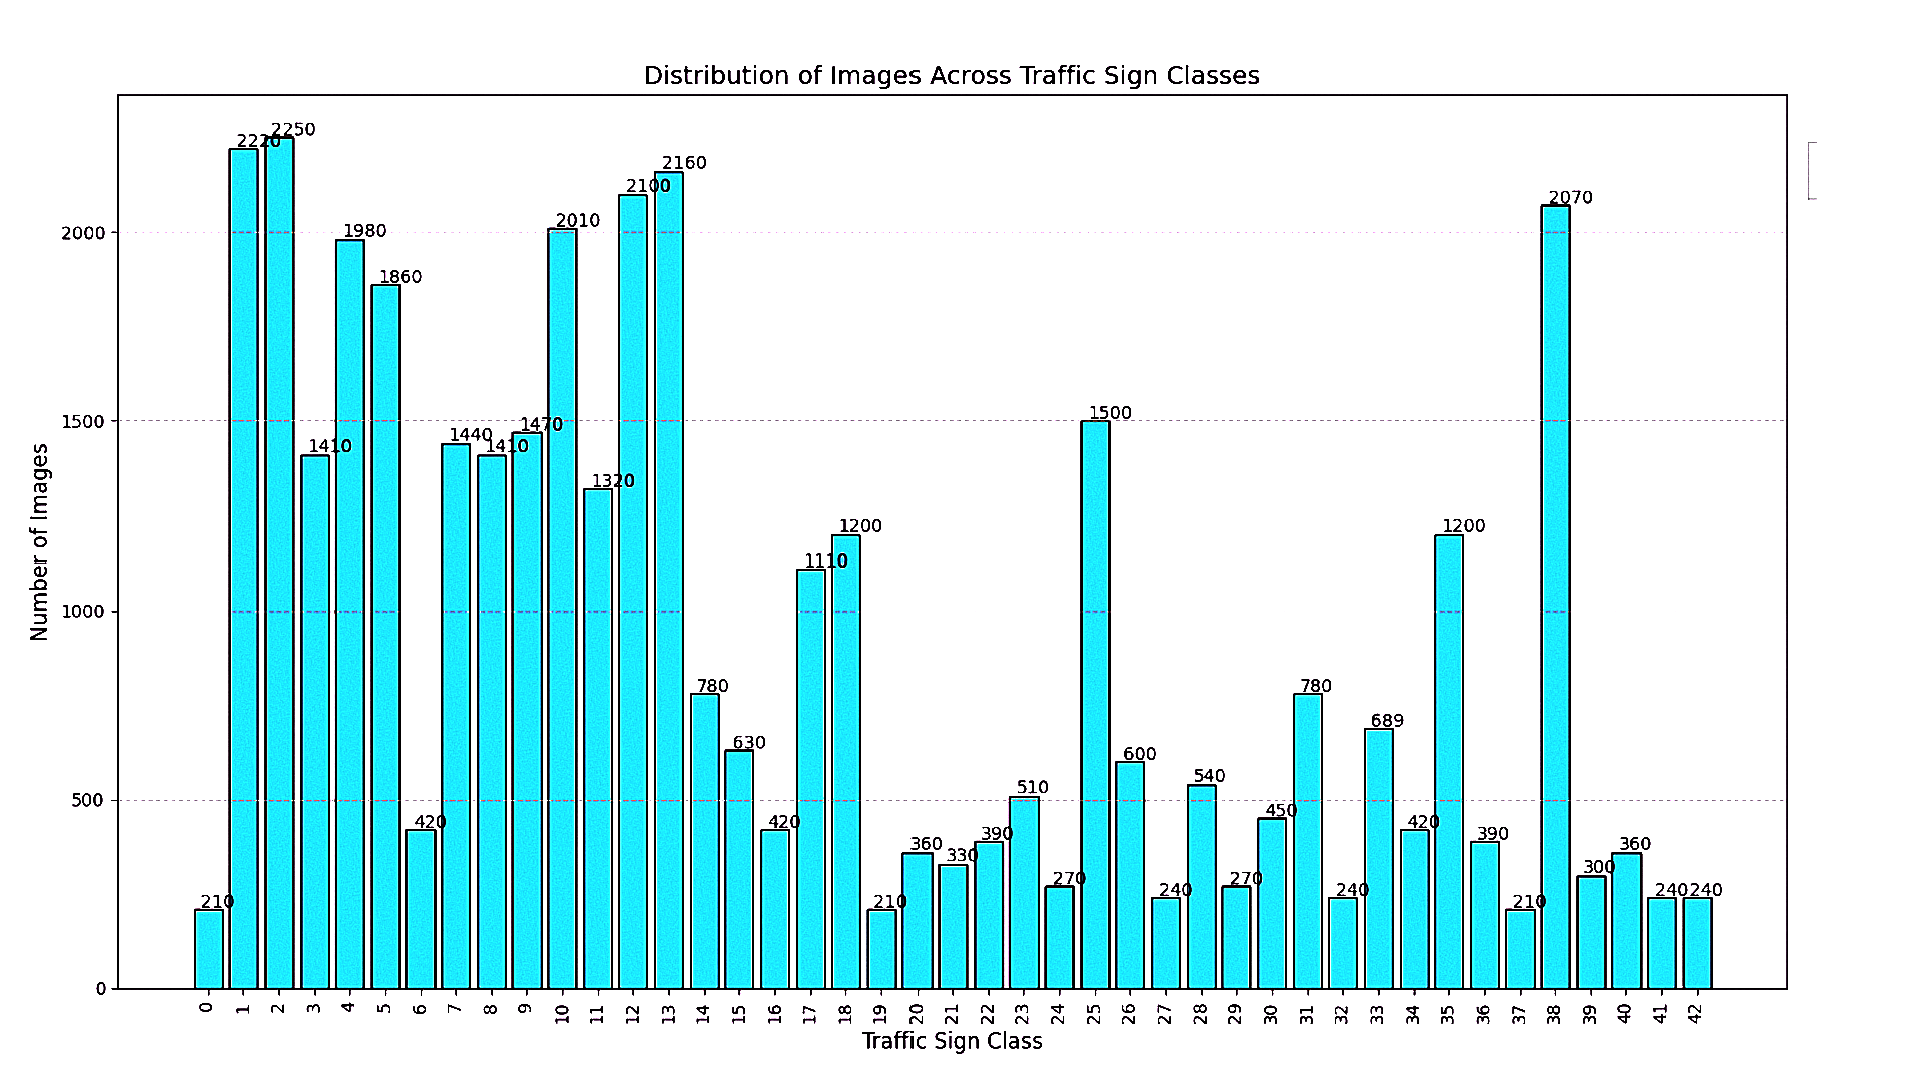
\includegraphics[width=1.2\textwidth]{bar_chart_unsorted}
    \caption{توزیع تعداد نمونه‌ها در کلاس‌ها (مرتب نشده) – این نمودار تعداد نمونه‌های موجود در هر کلاس را به ترتیب شماره کلاس‌ها (از 0 تا 42) نمایش می‌دهد. }
    \label{fig:class_dist_freq}
\end{figure}
\begin{figure}[H]
    \centering
    
\includegraphics[width=1\textwidth]{bar_chart_sorted}
    \caption{توزیع تعداد نمونه‌ها در کلاس‌ها (مرتب شده بر اساس تعداد) – در این نمودار، کلاس‌ها بر اساس تعداد نمونه‌های موجود مرتب شده‌اند تا توزیع داده‌ها به شکل واضح‌تری قابل مشاهده باشد.  }
    \label{fig:class_dist_freq}
\end{figure}











\subsubsection{تحلیل عدم تعادل داده‌ها}
اما همانطور که در بالا اشاره کردیم شیوه طراحی بصری علائم باعث شده که علائمی که شبیه هم هستند از لحاظ دسته بندی موضوعی هم بهم نزدیک تر باشند.پس می توانیم علائم را براساس معنا و جنس پیامی که انتقال می دهند که به نوعی هم میزان مهم بودن آن را نشان میدهد در زیر توزیع نمونه ها در دسته بندی های بصری و مفهومی که قبلا مطرح شد مشاهده می‌شود، توزیع نمونه‌ها در دسته‌بندی‌های مختلف از جمله رنگ، شکل، ترکیب شکل و رنگ و مفهوم علائم به وضوح نامتعادل است. این عدم توازن نشان‌دهنده فراوانی بسیار زیاد برخی دسته‌ها، مانند قرمز و سفید یا دایره، و فراوانی بسیار کم در دسته‌هایی مانند زرد و سفید با لوزی یا شش‌ضلعی است. چنین توزیعی می‌تواند مشکلات متعددی را ایجاد کند، از جمله سوگیری به سمت کلاس‌های پرتکرار، کاهش دقت در شناسایی کلاس‌های کم‌نمونه، و افت عملکرد مدل بر اساس معیارهای ارزیابی
 مانند \lr{Recall}\LTRfootnote{\lr{Recall}} و \lr{F1-Score}\LTRfootnote{\lr{F1-Score}}.

برای رفع این چالش‌ها، در این پژوهش مجموعه‌ای از تکنیک‌های افزایش داده و متوازن‌سازی به کار گرفته شده است. یکی از این تکنیک‌ها چرخش تصادفی\LTRfootnote{\lr{Random Rotation}} است که با اعمال زوایای مختلف بر تصاویر ورودی، مدل را قادر می‌سازد الگوهای چرخیده را نیز شناسایی کند. این روش با افزایش تنوع در مجموعه داده، به بهبود تعمیم‌پذیری مدل کمک کرده است. علاوه بر این، تغییر روشنایی و کنتراست\LTRfootnote{\lr{Color Jitter}} برای شبیه‌سازی شرایط نوری مختلف، مانند نور روز، شب و شرایط با روشنایی متغیر، به کار گرفته شده است. این تکنیک، مدل را در برابر تغییرات نوری مقاوم‌تر ساخته و دقت آن را در سناریوهای متنوع افزایش داده است.

همچنین، از تکنیک SMOTE\LTRfootnote{\lr{Synthetic Minority Over-sampling Technique}} برای تولید نمونه‌های مصنوعی در کلاس‌های کم‌نمونه استفاده شده است. این روش با افزایش تعداد نمونه‌های کلاس‌های نادر، توازن داده‌ها را بهبود بخشیده و شناسایی این کلاس‌ها را برای مدل تسهیل کرده است. علاوه بر این، وزن‌دهی در تابع هزینه\LTRfootnote{\lr{Weighted Loss}} نیز برای کاهش تأثیر کلاس‌های پرتکرار مورد استفاده قرار گرفته است. این تکنیک با اختصاص وزن‌های بالاتر به کلاس‌های کم‌نمونه در حین آموزش، مدل را به طور ضمنی به شناسایی این کلاس‌ها ترغیب کرده و عملکرد آن را در پیش‌بینی کلاس‌های نادر ارتقا داده است.

ترکیب این روش‌ها به افزایش تنوع داده‌ها و بهبود توازن میان کلاس‌ها منجر شده است. نتایج حاصل نشان می‌دهد که این استراتژی‌ها توانسته‌اند بر مشکلات ناشی از نامتوازن بودن داده‌ها غلبه کرده و مدلی پایدارتر، قابل‌اعتمادتر و با توانایی تعمیم بالاتر در مواجهه با داده‌های واقعی ارائه دهند. این رویکرد در مسائل عملی، به ویژه در کاربردهایی که عدم توازن داده‌ها می‌تواند به عملکرد مدل آسیب برساند


. \begin{figure}[H]
    \centering
    
\includegraphics[width=1\textwidth]{sample_ditribution}
    \caption{ این مجموعه نمودارها، توزیع نمونه‌ها را بر اساس رنگ، شکل، ترکیب شکل و رنگ و مفهوم علائم نمایش می‌دهد. نمودارها به وضوح نامتعادلی در توزیع داده‌ها را نشان می‌دهند؛ به‌طوری‌که برخی دسته‌ها مانند قرمز و سفید یا دایره بیشترین نمونه‌ها را دارند، در حالی که دسته‌هایی مانند زرد و سفید با لوزی یا شش‌ضلعی به‌ندرت دیده می‌شوند}
    \label{fig: sample_ditribution}
\end{figure}


. \begin{figure}[H]
    \centering
    
\includegraphics[width=1\textwidth]{cocept_based percentage}
    \caption{ نمودارها توزیع زیرکلاس‌های دسته‌بندی مفهومی را نمایش می‌دهند. نمودار بالا درصد نمونه‌های هر زیرکلاس را نسبت به کتگوری اصلی خود نشان می‌دهد، در حالی که نمودار پایین درصد نمونه‌های هر زیرکلاس را نسبت به کل دیتاست مقایسه می‌کند. این تحلیل به وضوح نامتوازن بودن برخی زیرکلاس‌ها را در هر دو
    مقیاس نشان می‌دهد،}
    \label{fig: cocept_based percentage}
\end{figure}
\section{متعادل‌سازی داده‌ها با استفاده از تکنیک‌های افزایش داده}

برای رفع عدم توازن در توزیع کلاس‌ها، از روش‌های افزایش داده مانند \lr{SMOTE}\LTRfootnote{Synthetic Minority Over-sampling Technique} استفاده شد. این روش با تولید نمونه‌های مصنوعی، داده‌های کلاس‌های اقلیت را افزایش داده و توزیع را متعادل می‌کند. علاوه بر آن، تکنیک‌های دیگری شامل چرخش\LTRfootnote{Rotation}، تغییر نور و روشنایی\LTRfootnote{Brightness Adjustment}، جابجایی\LTRfootnote{Translation}، افزودن نویز\LTRfootnote{Adding Noise} و تغییر مقیاس\LTRfootnote{Scaling} به کار گرفته شدند. 

این اقدامات منجر به بهبود توزیع کلاس‌ها و افزایش تنوع ویژگی‌ها شد. نتایج نشان داد که مدل پس از اعمال این روش‌ها دقت بیشتری در پیش‌بینی داده‌های اقلیت داشته و توانایی آن در مواجهه با شرایط مختلف افزایش یافته است. استفاده از این تکنیک‌ها به وضوح توانست عدم توازن داده‌ها را کاهش داده و کارایی مدل را بهبود بخشد.


\begin{figure}[H]
    \centering
    \begin{subfigure}{0.3\textwidth}
        
\includegraphics[width=\linewidth]{sample_augmented_1}
        \caption{نمونه 1}
    \end{subfigure}
    \begin{subfigure}{0.3\textwidth}
        
\includegraphics[width=\linewidth]{sample_augmented_2}
        \caption{نمونه 2}
    \end{subfigure}
    
    \caption{نمونه‌هایی از تصاویر افزوده شده}
    \label{fig:augmented_samples}
\end{figure}

همچنین، نمودار زیر توزیع کلاس‌ها را قبل و بعد از افزایش داده مقایسه می‌کند.

\begin{figure}[H]
    \centering
    
\includegraphics[width=1\textwidth]{class_distribution_comparison}
    \caption{توزیع کلاس‌ها قبل و بعد از افزایش داده}
    \label{fig:class_distribution}
\end{figure}



\begin{table}[h]
\centering
\renewcommand{\arraystretch}{1} % تنظیم فاصله عمودی سلول‌ها
\setlength{\tabcolsep}{8pt}      % تنظیم فاصله افقی سلول‌ها
\begin{tabular}{|l|l|l|}
\hline
\textbf{آمار}                                  & \textbf{قبل از افزایش داده}                      & \textbf{بعد از افزایش داده}                    \\ \hline
\lr{Max Image Count}                          & \lr{2250}                                      & \lr{2250}                                      \\ \hline
\lr{Min Image Count}                          & \lr{210}                                       & \lr{2250}                                      \\ \hline
\lr{Imbalance Ratio (Max / Min)}             & \lr{10.71}                                    & \lr{1.00}                                     \\ \hline
\lr{Average Image Count per Class}           & \lr{1036.58}                                  & \lr{2250.00}                                  \\ \hline
\lr{Standard Deviation of Image Count}       & \lr{790.44}                                   & \lr{0.00}                                     \\ \hline
\end{tabular}
\caption{ویژگی های آماری تصاویر قبل و بعد از افزایش داده در سطح کلاس}
\label{tab:statistics}
\end{table}

برای توازن داده‌ها از تکنیک‌هایی نظیر چرخش تصادفی، انتقال، وارونگی افقی و
تکنیک‌های افزایش داده به طور مؤثری داده‌ها را متوازن کرده و نسبت عدم توازن را از \lr{10.71} به \lr{1.00} کاهش داده‌اند. این امر باعث می‌شود مدل آموزش‌دیده بر روی این داده‌ها کمتر به کلاس‌هایی با تعداد بیشتر تصاویر گرایش داشته باشد.
\subsection{متعادل‌سازی در سطح دسته‌بندی‌های معنایی و بصری}

برای بهبود تعادل داده‌ها، فرآیند تعادل‌سازی نه تنها در سطح کلاس‌ها، بلکه در سطح دسته‌بندی‌های اصلی و زیرمجموعه‌های معنایی و بصری اعمال گردید. 

جدول \ref{tab:comparison} تعداد تصاویر قبل و بعد از افزایش داده را بر اساس دسته‌بندی‌های اصلی شامل رنگ، شکل و مفهوم مقایسه می‌کند. این جدول نشان‌دهنده تغییرات در توزیع داده‌ها بین این دسته‌بندی‌ها است. 

در ادامه، جدول \ref{tab:combined_ratios} به صورت جزئی‌تر به بررسی نسبت‌های عدم تعادل در زیرگروه‌های مفهومی می‌پردازد و تغییرات پیش و پس از افزایش داده را برای این زیرگروه‌ها نشان می‌دهد. این مقایسه به وضوح میزان تأثیر فرآیند افزایش داده در متعادل‌سازی زیرگروه‌های مفهومی را مشخص می‌کند.


\begin{table}[h!]
\centering
\renewcommand{\arraystretch}{0.8} % Reduce row height
\scriptsize % Reduce font size
\resizebox{\textwidth}{!}{%
\begin{tabular}{|p{4cm}|p{3cm}|p{3cm}|}
\hline
\textbf{دسته‌بندی} & \textbf{قبل از افزوده‌سازی} & \textbf{بعد از افزوده‌سازی} \\ \hline
\multicolumn{3}{|c|}{\textbf{دسته‌بندی‌های مبتنی بر رنگ}} \\ \hline
زیرگروه قرمز و سفید & \lr{10.71} & \lr{1.66} \\ \hline
زیرگروه سیاه و سفید & \lr{1.75} & \lr{1.02} \\ \hline
زیرگروه زرد و سیاه & \lr{3.85} & \lr{1.21} \\ \hline
زیرگروه زرد و سفید & \lr{1.00} & \lr{1.00} \\ \hline
زیرگروه آبی و سفید & \lr{9.86} & \lr{1.33} \\ \hline
\multicolumn{3}{|c|}{\textbf{دسته‌بندی‌های مبتنی بر شکل}} \\ \hline
زیرگروه دایره & \lr{10.71} & \lr{1.96} \\ \hline
زیرگروه مثلث & \lr{7.14} & \lr{1.29} \\ \hline
زیرگروه لوزی & \lr{1.00} & \lr{1.00} \\ \hline
زیرگروه مثلث وارونه & \lr{1.00} & \lr{1.00} \\ \hline
زیرگروه شش‌ضلعی & \lr{1.00} & \lr{1.00} \\ \hline
\multicolumn{3}{|c|}{\textbf{دسته‌بندی‌های مبتنی بر مفهوم}} \\ \hline
زیرگروه علائم محدودیت سرعت & \lr{10.71} & \lr{1.59} \\ \hline
زیرگروه علائم بازدارنده دیگر & \lr{4.79} & \lr{1.21} \\ \hline
زیرگروه علائم رفع محدودیت & \lr{1.75} & \lr{1.02} \\ \hline
زیرگروه علائم اجباری & \lr{9.86} & \lr{1.33} \\ \hline
زیرگروه علائم خطر & \lr{7.14} & \lr{1.29} \\ \hline
زیرگروه علائم منحصربه‌فرد & \lr{2.77} & \lr{1.25} \\ \hline
\end{tabular}}
\caption{جدول مقایسه‌ای نسبت عدم‌تعادل قبل و بعد افزایش داده}
\label{tab:comparison}
\end{table}

\clearpage
\vspace{-1cm}
\begin{table}[h!]
\centering
\renewcommand{\arraystretch}{0.9} % Reduce row height
\scriptsize % Reduce font size
\resizebox{\textwidth}{!}{%
\begin{tabular}{|p{3cm}|p{3cm}|p{2cm}|p{2cm}|p{2.5cm}|p{2.5cm}|}
\hline
\textbf{گروه اصلی} & \textbf{زیرگروه} & \textbf{تعداد کل} & \textbf{بیشترین تعداد} & \textbf{کمترین تعداد} & \textbf{نسبت عدم تعادل (نهایی)} \\ \hline
علائم محدودیت سرعت & سرعت کم & \lr{4680} & \lr{2945} & \lr{2220} & \lr{1.32658} \\ \hline
علائم محدودیت سرعت & سرعت متوسط & \lr{5250} & \lr{1980} & \lr{1410} & \lr{1.40426} \\ \hline
علائم محدودیت سرعت & سرعت زیاد & \lr{2850} & \lr{1440} & \lr{1410} & \lr{1.02128} \\ \hline
علائم بازدارنده دیگر & محدودیت وسیله نقلیه & \lr{3480} & \lr{2010} & \lr{1470} & \lr{1.36735} \\ \hline
علائم بازدارنده دیگر & ممنوعیت‌های عمومی & \lr{1050} & \lr{630} & \lr{420} & \lr{1.5} \\ \hline
علائم رفع محدودیت & رفع محدودیت سرعت & \lr{660} & \lr{420} & \lr{240} & \lr{1.75} \\ \hline
علائم رفع محدودیت & رفع محدودیت عبور & \lr{480} & \lr{240} & \lr{240} & \lr{1} \\ \hline
علائم اجباری & علائم جهت‌یابی اولیه & \lr{2309} & \lr{1200} & \lr{689} & \lr{1.74165} \\ \hline
علائم اجباری & علائم جهت‌یابی ثانویه & \lr{3330} & \lr{2070} & \lr{1680} & \lr{1.23214} \\ \hline
علائم خطر & هشدارهای عمومی & \lr{1650} & \lr{1200} & \lr{750} & \lr{1.6} \\ \hline
علائم خطر & خطرات هندسی جاده & \lr{1350} & \lr{510} & \lr{270} & \lr{1.88889} \\ \hline
علائم خطر & شرایط سرعت و سطح & \lr{660} & \lr{390} & \lr{270} & \lr{1.44444} \\ \hline
علائم خطر & خطرات عابران و ترافیکی & \lr{2880} & \lr{1500} & \lr{900} & \lr{1.66667} \\ \hline
علائم خطر & خطرات محیطی & \lr{2100} & \lr{1320} & \lr{780} & \lr{1.69231} \\ \hline
علائم خطر & مناطق ساخت و ساز & \lr{330} & \lr{330} & \lr{330} & \lr{1} \\ \hline
علائم منحصربه‌فرد & علائم اولویت و توقف & \lr{2940} & \lr{2160} & \lr{1379} & \lr{1.56635} \\ \hline
علائم منحصربه‌فرد & ممنوعیت‌ها و محدودیت‌ها & \lr{1110} & \lr{1110} & \lr{1110} & \lr{1} \\ \hline
علائم منحصربه‌فرد & علائم هشداردهنده & \lr{2100} & \lr{2100} & \lr{2100} & \lr{1} \\ \hline
\end{tabular}}
\caption{نسبت‌های عدم تعادل قبل و بعد از افزوده‌سازی برای هر زیرگروه}
\label{tab:combined_ratios}
\end{table}
\section{پیش‌پردازش داده‌ها}
در این بخش، فرآیند آماده‌سازی داده‌ها برای استفاده در مدل توضیح داده می‌شود. پیش‌پردازش داده‌ها مرحله‌ای کلیدی در طراحی و توسعه‌ی مدل‌های یادگیری عمیق\LTRfootnote{Deep Learning} است و بهبود دقت و کارایی مدل به طور مستقیم به کیفیت این مرحله وابسته است. در این پروژه، فرآیند پیش‌پردازش شامل سه مرحله‌ی اصلی به شرح زیر است:
\newline
ابتدا تمامی تصاویر موجود در مجموعه داده به ابعاد ثابت \lr{32}×\lr{32} پیکسل تغییر اندازه داده شدند. تغییر اندازه\LTRfootnote{Resizing} نه تنها سبب تسهیل پردازش داده‌ها توسط مدل می‌شود، بلکه باعث یکنواختی داده‌های ورودی\LTRfootnote{Input Data Uniformity} می‌گردد.

در مرحله‌ی دوم، مقادیر پیکسل‌های تصاویر به منظور بهبود فرآیند یادگیری به بازه‌ی \lr{[0,1]} نرمال‌سازی\LTRfootnote{Normalization} شدند. این نرمال‌سازی با تقسیم مقادیر پیکسل‌ها بر مقدار حداکثری ممکن (\lr{255}) انجام شد. این عمل باعث شد داده‌ها از لحاظ مقیاس\LTRfootnote{Scale} در سطحی متناسب با نیازهای مدل قرار گیرند. به عنوان نکته‌ی قابل توجه، این عملیات معکوس‌پذیر است؛ یعنی با انجام معکوس نرمال‌سازی\LTRfootnote{Inverse Normalization} (ضرب داده‌های نرمال‌شده در \lr{255})، می‌توان تصویر اولیه را با دقت بالا بازسازی کرد.
\ref{fig:reduced-height-image}.


\begin{figure}[ht]
    \centering
    
\includegraphics[height=0.8\textwidth]{normalized_example} % Replace 'normalized_example' with your image file name
    \caption{نمونه تصاویر قبل و بعد نرمال‌سازی. این تصاویر شامل نمونه‌هایی از تصاویر اصلی، تصاویر بعد از نرمال‌سازی و همچنین تصاویر بازسازی‌شده با استفاده از نرمال‌سازی معکوس هستند.}
    \label{fig:reduced-height-image}
\end{figure}


در این تحقیق، از سه مدل مختلف MobileNet، ResNet و EfficientNet برای ارزیابی عملکرد در پردازش تصاویر استفاده شده است. در مرحله‌ی سوم، تصاویر پیش‌پردازش‌شده به عنوان ورودی، به‌طور جداگانه بر روی هر یک از این مدل‌ها آزمایش شدند.
مدل MobileNetV2 (\lr{MobileNetV2 Architecture}) به دلیل طراحی سبک و توانایی بالا در یادگیری ویژگی‌ها در سیستم‌های کم‌منبع (\lr{Resource-Constrained Systems}) انتخاب شد. مدل ResNet (\lr{Residual Networks}) به‌عنوان یک معماری عمیق با امکان اتصال مستقیم لایه‌ها (\lr{Residual Connections}) برای یادگیری بهتر ویژگی‌های پیچیده مورد استفاده قرار گرفت. در نهایت، مدل EfficientNet (\lr{EfficientNet Architecture}) به دلیل بهره‌وری بالا در استفاده از منابع محاسباتی و دقت بالا در مقایسه با مدل‌های مشابه، برای انجام آزمایشات در نظر گرفته شد.
برای نمایش مراحل پیش‌پردازش، نمونه‌هایی از تصاویر اولیه، تصاویر پس از نرمال‌سازی، و همچنین تصاویر بازسازی‌شده با استفاده از نرمال‌سازی معکوس ارائه خواهند شد. این تصاویر در جدول زیر قرار داده شده‌اند و به‌صورت بصری تأثیر مراحل پیش‌پردازش و قابلیت بازسازی تصویر اولیه را نشان می‌دهند.



\section{مقایسهٔ عملکرد مدل‌ها}

در این بخش، عملکرد سه مدل مختلف شامل \lr{MobileNet}، \lr{EfficientNet} و \lr{ResNet} در شناسایی کلاس‌های مختلف با استفاده از داده‌های پیش‌پردازش‌شده و خام بررسی خواهد شد. هر مدل در دو حالت آموزش داده شده است: حالت اول با استفاده از داده‌های خام و حالت دوم با استفاده از داده‌های پیش‌پردازش‌شده. برای هر کدام از این شش حالت، نتایج به کمک معیارهای مختلف مانند دقت، فراخوانی و معیار \lr{F1} مقایسه خواهند شد. علاوه بر این، \lr{Confusion Matrices} برای هر مدل و هر حالت نیز ارائه شده‌اند تا دیدگاه کاملی از عملکرد مدل‌ها در اختیار قرار گیرد.

\subsection{مقایسه معیارهای عملکرد مدل‌ها}

\begin{table}[H]
\centering
\renewcommand{\arraystretch}{0.8} % Reduce row height
\scriptsize % Reduce font size
\resizebox{\textwidth}{!}{%
\begin{tabular}{|p{3cm}|p{2.5cm}|p{2.5cm}|p{2.5cm}|p{2.5cm}|p{2.5cm}|}
\hline
\lr{\textbf{Model}} & \lr{\textbf{Data Type}} & \lr{\textbf{Accuracy}} & \lr{\textbf{Precision}} & \lr{\textbf{Recall}} & \lr{\textbf{F1 Score}} \\ \hline
\lr{MobileNetV2} & \lr{Raw} & \lr{68.107680} & \lr{0.866821} & \lr{0.681077} & \lr{0.709799} \\ \hline
\lr{MobileNetV2} & \lr{Preprocessed} & \lr{96.286619} & \lr{0.967904} & \lr{0.962866} & \lr{0.961895} \\ \hline
\lr{ResNet18} & \lr{Raw} & \lr{34.623911} & \lr{0.924542} & \lr{0.346239} & \lr{0.441328} \\ \hline
\lr{ResNet18} & \lr{Preprocessed} & \lr{96.310372} & \lr{0.966514} & \lr{0.963104} & \lr{0.962967} \\ \hline
\lr{EfficientNet} & \lr{Raw} & \lr{26.682502} & \lr{0.656621} & \lr{0.266825} & \lr{0.328322} \\ \hline
\lr{EfficientNet} & \lr{Preprocessed} & \lr{97.418844} & \lr{0.976981} & \lr{0.974188} & \lr{0.972184} \\ \hline
\end{tabular}%
}
\caption{مقایسهٔ عملکرد مدل‌های مختلف در داده‌های خام و پیش‌پردازش‌شده}
\label{tab:comparison-models}
\end{table}


در این جدول، مقایسه‌ای بین مدل‌های \lr{MobileNet}، \lr{EfficientNet} و \lr{ResNet} در دو حالت داده (پیش‌پردازش‌شده و خام) از نظر دقت، فراخوانی و معیار \lr{F1} انجام شده است. همچنین، تفاوت میان معیار \lr{F1} هر مدل در حالت‌های مختلف نیز در جدول آورده شده است.

نتایج آزمون \lr{ANOVA} نشان داد که تفاوت‌های مشاهده‌شده بین مدل‌ها در داده‌های خام و پیش‌پردازش‌شده از نظر آماری معنادار هستند (با \(\text{F-statistic} = 17.77\) و \(\text{p-value} = 0.0135\)). این نتایج حاکی از تأثیر مثبت پیش‌پردازش بر عملکرد مدل‌ها است. در عین حال، \lr{MobileNet} در داده‌های خام عملکرد بهتری نسبت به مدل‌های دیگر داشت. این عملکرد بهتری می‌تواند به معماری سبک و کارآمد \lr{MobileNet} مربوط باشد. این مدل از \lr{Depthwise Separable Convolutions} برای کاهش پیچیدگی محاسباتی و افزایش کارایی استفاده می‌کند، که موجب می‌شود بتواند حتی در داده‌های خام و بدون پیش‌پردازش، ویژگی‌های عمومی تصاویر را به خوبی استخراج کند. همچنین، طراحی \lr{MobileNet} به گونه‌ای است که نیاز به توان محاسباتی کمتری دارد و در مواجهه با داده‌های ساده‌تر یا کم‌حجم‌تر بهتر عمل می‌کند، در حالی که مدل‌های پیچیده‌تر مانند \lr{ResNet} و \lr{EfficientNet} به داده‌های پیش‌پردازش‌شده و پیچیده‌تری نیاز دارند تا عملکرد مطلوبی داشته باشند.




\subsection{ماتریس‌های اشتباه (\lr{Confusion Matrices})}

در این بخش، \lr{Confusion Matrices} برای هر مدل در دو حالت داده (پیش‌پردازش‌شده و خام) ارائه شده است. این ماتریس‌ها به‌طور دقیق نحوه عملکرد مدل‌ها را در پیش‌بینی کلاس‌ها نشان می‌دهند. شکل‌های زیر، \lr{Confusion Matrices} مربوط به هر مدل را در هر دو حالت داده نشان می‌دهند.

\begin{figure}[H]
\centering
\begin{minipage}{0.48\textwidth}
    \centering
    
\includegraphics[width=0.7\textwidth, height=0.25\textheight]{mobile_raw}
    \caption{\tiny Confusion Matrix of \lr{MobileNet} with Raw Data}
    \label{subchart1}
\end{minipage} \hfill
\begin{minipage}{0.48\textwidth}
    \centering
    
\includegraphics[width=0.7\textwidth, height=0.25\textheight]{mobile_Aug}
    \caption{\tiny Confusion Matrix of \lr{MobileNet} with Preprocessed Data}
    \label{subchart2}
\end{minipage}

\vspace{0.5cm}

\begin{minipage}{0.48\textwidth}
    \centering
    
\includegraphics[width=0.7\textwidth, height=0.25\textheight]{eff_raw}
    \caption{\tiny Confusion Matrix of \lr{EfficientNet} with Raw Data}
    \label{subchart3}
\end{minipage} \hfill
\begin{minipage}{0.48\textwidth}
    \centering
    
\includegraphics[width=0.7\textwidth, height=0.25\textheight]{resNet_raw}
    \caption{\tiny Confusion Matrix of \lr{EfficientNet} with Preprocessed Data}
    \label{subchart4}
\end{minipage}

\vspace{0.5cm}

\begin{minipage}{0.48\textwidth}
    \centering
    
\includegraphics[width=0.7\textwidth, height=0.25\textheight]{resNet_raw}
    \caption{\tiny Confusion Matrix of \lr{ResNet} with Raw Data}
    \label{subchart5}
\end{minipage} \hfill
\begin{minipage}{0.48\textwidth}
    \centering
    
\includegraphics[width=0.7\textwidth, height=0.25\textheight]{resNet_aug}
    \caption{\tiny Confusion Matrix of \lr{ResNet} with Preprocessed Data}
    \label{subchart6}
\end{minipage}
\caption{\tiny Confusion Matrices of the \lr{Models}}
\label{fig:confusion-matrices}
\end{figure}

\section{
نتایج تاثیر شبیه سازی شرایط جوی مختلف بر روی تصاویر }

در بخش‌های قبلی توضیح داده شد که داده‌ها به‌طور متوازن و با توزیع نا یکسان آماده شدند. برای این منظور، در راستای اصلاح توزیع داده‌ها و رسیدن به تعادل مطلوب، شرایط مختلفی مورد بررسی قرار گرفت. این شرایط شامل تغییرات در تعداد کلاس‌ها، تنوع اشکال و رنگ‌ها، و تغییرات معانی علائم بود. هدف اصلی این بخش، شبیه‌سازی شرایط جوی واقعی بود تا بتوانیم اثر یادگیری مدل هوش مصنوعی را بر اساس داده‌های اصلاح‌شده ارزیابی کنیم. 
هدف اصلی این آزمایش‌ها، آموزش مدل به‌گونه‌ای بود که بتواند در شرایط جوی مختلف (مانند مه، باران، برف و...) عملکرد مناسبی داشته باشد. به‌طور خاص، سعی کردیم تأثیرات شرایط جوی نظیر تغییر رنگ به‌دلیل نور خورشید، سفید شدن تابلوها با برف، و کاهش دید در شرایط مه و باران را شبیه‌سازی کنیم. این‌گونه مدل می‌تواند عملکرد انسانی را که به‌طور طبیعی این تغییرات را تشخیص می‌دهد، شبیه‌سازی کند. 

\begin{figure}[h] \centering 
\includegraphics[width=0.8\textwidth]{effect} \caption{تصویر نمونه هایی از اعمال باران ، برف ، مه ، باد و نور زیاد خورشید را مشاهده میکنید } \label{fig:effects} \end{figure}

\subsection*{پیاده سازی و شرایط آزمایشی}
در این مرحله، برای بررسی دقیق‌تر عملکرد مدل، شرایط جوی مختلف به‌صورت مستقل بر روی داده‌ها اعمال شد. به‌عنوان مثال، در شرایط بارانی تنها افکت باران به تصاویر اعمال شد و هیچ‌گونه شرایط جوی دیگر مانند باد در نظر گرفته نشد. هدف در این مرحله، ساده‌سازی شرایط آزمایشی بود تا بتوانیم اثر هر شرایط جوی به‌طور مستقل بررسی کنیم.هر چند که در خیلی از حالت ها احتمال وجود بیش از یک مورد از این حالت ها وجود دارد . این کار به ما این امکان را می‌دهد که مدل را در برابر هر یک از این شرایط به‌طور مجزا تست کرده و تأثیر آنها را به‌دقت اندازه‌گیری کنیم. 

\subsection{نتایج و مقایسه }

در اینجا درک تاثیر یادگیری از این تصاویر ، اول مدل آموزش دیده با داده های اولیه را با یک مجموعه آزمایشی تست کردیم که شامل حدود \lr{15%} داده های فیلتر شده بود . نتایج آن به شکل زیر بود 

در آزمایش اول که برای آموزش مدل با داده‌های اولیه انجام شد، نتایج به‌دست‌آمده برای دقت آموزش 0.6745 و خطا 1.0653 بود. همچنین برای داده‌های اعتبارسنجی، دقت 0.6929 و خطا 0.9965 به‌دست آمد، و بالاترین دقت اعتبارسنجی 0.7029 بود. در تحلیل این نتایج، مشاهده شد که عملکرد مدل نسبت به آزمایشات قبلی که بر روی داده‌های معمولی انجام شده بود، ضعیف‌تر است و این ممکن است به دلایلی مانند تغییرات داده‌ها یا پارامترهای مدل مرتبط باشد. در آزمایش دوم، حدود 20 درصد از تصاویر به‌طور تصادفی فیلتر شدند و پس از آموزش مدل، نتایج به‌صورت زیر به‌دست آمد: دقت آموزش 0.839 و خطا 0.9388 و برای داده‌های اعتبارسنجی، دقت 0.8102 و خطا 0.8249 به‌دست آمد. همچنین، بالاترین دقت اعتبارسنجی در این آزمایش به 0.839 رسید.



تأثیرات شرایط جوی مختلف را بر روی عملکرد مدل دید. این نتایج نشان می‌دهند که مدل توانسته است تا حد زیادی با شرایط جوی مختلف سازگار شود و عملکردی مشابه انسان در تشخیص تغییرات محیطی ارائه دهد. 
\subsection{پیاده‌سازی فیلترهای محیطی در تصاویر و نحوه عملکرد آن‌ها} 
برای پیاده‌سازی فیلترهای مختلف محیطی بر روی تصاویر و بررسی عملکرد آن‌ها، از کتابخانه‌ی \LTRfootnote{albumentations} برای اعمال تکنیک‌های افزایش داده استفاده کردیم. برای شبیه‌سازی شرایط مختلف محیطی بر روی تصاویر، از مجموعه‌ای از فیلترها استفاده می‌شود. به‌عنوان مثال، برای شبیه‌سازی باران، از دو فیلتر بلور گوسی و نویز گوسی بهره می‌بریم. فیلتر بلور گوسی به‌طور خاص برای شبیه‌سازی افکت‌های مه‌آلود یا بارانی به‌کار می‌رود، زیرا با اعمال تاری بر روی تصویر، جزئیات کمتری قابل مشاهده خواهد بود که مشابه به محدود شدن دید در هنگام بارش باران است. فیلتر نویز گوسی نیز برای اضافه کردن نویز به تصویر استفاده می‌شود که مشابه باران است و باعث ایجاد ناپایداری و تاری در تصویر می‌شود، و به مدل کمک می‌کند تا ویژگی‌های مهم را حتی در شرایط نویزی شبیه‌سازی‌شده یاد بگیرد. 
در شبیه‌سازی برف، از فیلتر تصادفی برف استفاده می‌شود. این فیلتر باعث اضافه کردن افکت برف به تصویر می‌شود و با استفاده از پارامترهایی مانند ضریب روشنایی برای روشن‌تر کردن برف‌ها و حد پایین و حد بالای نقطه برف برای تنظیم درصد پوشش برف، تصویر را تغییر می‌دهد. 
برای شبیه‌سازی مه، از فیلتر بلور گوسی بیشتر استفاده می‌شود تا تصویری که تحت تأثیر مه تاری می‌خورد، شبیه‌سازی شود. این فیلتر باعث کاهش کنتراست و وضوح تصویر می‌شود، که به‌طور دقیق شرایط دید در مه را شبیه‌سازی می‌کند. 
در شبیه‌سازی باد، فیلتر تغییر الاستیک به‌کار می‌رود که باعث ایجاد انحراف در تصویر می‌شود. این تغییرات الاستیک به‌طور مشابه باعث شبیه‌سازی حرکت اشیاء تحت تأثیر باد می‌گردد. 
در نهایت، برای شبیه‌سازی نور خورشید، فیلتر تغییر روشنایی و کنتراست به تصویر اعمال می‌شود. این تغییرات می‌تواند تأثیرات نور خورشید را در تصاویر شبیه‌سازی کند و باعث ایجاد تابش یا سایه‌ها در تصویر شود. 
این فیلترها به‌طور کلی برای شبیه‌سازی شرایط مختلف محیطی و آموزش مدل‌ها در شرایط واقعی استفاده می‌شوند تا عملکرد بهتری در محیط‌های واقعی داشته باشند. 
\subsection{نحوه اجرای فیلترها}
در کد ارائه‌شده، ابتدا شرایط محیطی مختلفی همچون باران، برف، مه، باد و نور خورشید در یک دیکشنری به نام \lr{conditions} تعریف می‌شوند. سپس، بر اساس مقادیر این شرایط، فیلترهای مناسب به تصویر اعمال می‌گردند. برای هرکدام از این شرایط، فیلترهای مرتبط به‌عنوان افزونه‌هایی به یک پایپلاین افزایش داده اضافه می‌شوند. در نهایت، تصویر تحت تأثیر این تغییرات قرار می‌گیرد و به‌طور مصنوعی شرایط محیطی مختلف را شبیه‌سازی می‌کند. این فرآیند به‌منظور آموزش مدل‌ها تحت شرایط متنوع محیطی انجام می‌شود، تا مدل‌ها قادر به یادگیری ویژگی‌ها و الگوهای مختلف در محیط‌های چالش‌برانگیز باشند.
\subsection{خلاصه عملکرد فیلترها}
این فیلترها به‌طور دقیق شرایط محیطی مختلف را به تصویر اعمال می‌کنند:
\textbf{باران:} با استفاده از اعمال تاری و اضافه کردن نویز گوسی شبیه‌سازی می‌شود، که موجب کاهش وضوح و ایجاد افکت‌های مشابه باران می‌شود.
\textbf{برف:} با اعمال افکت‌های برفی و تغییرات در روشنایی تصویر شبیه‌سازی می‌شود. این فرآیند برای شبیه‌سازی تصاویر برفی با ویژگی‌های خاص همچون پراکندگی نور در برف و تغییرات کنتراست طراحی شده است.
\textbf{مه:} با استفاده از افزایش تاری تصویر (مانند بلور گوسی) شبیه‌سازی می‌شود، که باعث کاهش کنتراست و وضوح تصویر می‌گردد، مشابه شرایط دید در مه.
\textbf{باد:} با اعمال تغییرات الاستیک در تصویر شبیه‌سازی می‌شود، که به‌طور موثر انحرافات ناشی از حرکت و وزش باد در محیط را نشان می‌دهد.
\textbf{نور خورشید:} با تغییرات در روشنایی و کنتراست تصویر، به‌گونه‌ای که تأثیرات تابش نور خورشید و سایه‌ها را شبیه‌سازی کند.
این فیلترها نه‌تنها به شبیه‌سازی شرایط محیطی متنوع کمک می‌کنند، بلکه باعث می‌شوند تا مدل‌ها به‌طور مؤثرتری تحت شرایط محیطی مختلف آموزش ببینند. این امر موجب می‌شود که مدل‌ها در دنیای واقعی عملکرد بهتری داشته باشند و توانایی بالاتری در پیش‌بینی و تحلیل داده‌ها از خود نشان دهند.


